% Results section, included from report.tex. All tables are generated by
% scripts/make_report_tables.py from output/scenarios/scenario-results.json.

\subsubsection*{A. Service acceptance}

Table~\ref{tab:acc} and Figure~\ref{fig:acc} give the hold-out acceptance for
every scenario. The main scenarios are all heavy load: offered demand at 90\%,
100\% and 110\% of the network's compute capacity. Updated FPPVS hits the 70\%
target in all six main scenarios. Its mean acceptance goes from \fppvsMinAcc\%
(\fppvsWorstScenario) to \fppvsMaxAcc\%, with an average of \fppvsMeanAcc\%. The
lowest value in any single seed was \fppvsLowestRun\%, so the target holds run
by run too, not just on average.

\begin{table}[H]
\centering\footnotesize
\setlength{\tabcolsep}{4pt}
\caption{Hold-out service acceptance (\%), mean $\pm$ standard deviation over
\numSeeds{} seeds. Best value per row in bold.}
\label{tab:acc}
\begin{tabular}{lccccc}
\toprule
Scenario (topology, load) & Updated (ours) & Original FPPVS & 2022 adaptation & Greedy & Random \\
\midrule
Backbone 0.9 & \textbf{91.0 $\pm$ 3.6} & 77.0 $\pm$ 2.1 & 47.8 $\pm$ 7.6 & 58.7 $\pm$ 4.4 & 57.4 $\pm$ 4.0 \\
Backbone 1 & \textbf{86.4 $\pm$ 3.7} & 72.9 $\pm$ 2.4 & 44.5 $\pm$ 6.5 & 53.4 $\pm$ 5.1 & 55.3 $\pm$ 3.4 \\
Backbone 1.1 & \textbf{80.8 $\pm$ 3.8} & 67.7 $\pm$ 3.1 & 43.0 $\pm$ 10.4 & 51.9 $\pm$ 4.9 & 52.9 $\pm$ 3.3 \\
Metro 0.9 & \textbf{86.1 $\pm$ 2.9} & 73.6 $\pm$ 3.6 & 53.1 $\pm$ 9.3 & 56.3 $\pm$ 3.1 & 56.6 $\pm$ 3.0 \\
Metro 1 & \textbf{81.3 $\pm$ 3.5} & 69.6 $\pm$ 3.6 & 49.4 $\pm$ 9.7 & 51.8 $\pm$ 3.6 & 52.6 $\pm$ 3.0 \\
Metro 1.1 & \textbf{76.6 $\pm$ 2.5} & 65.6 $\pm$ 3.2 & 50.1 $\pm$ 5.2 & 48.8 $\pm$ 1.9 & 50.9 $\pm$ 3.1 \\
\midrule \multicolumn{6}{l}{\emph{Other load levels (light load and overload)}} \\
Backbone 0.5 & \textbf{99.6 $\pm$ 0.4} & 91.2 $\pm$ 2.3 & 68.1 $\pm$ 5.4 & 72.1 $\pm$ 5.8 & 73.2 $\pm$ 4.5 \\
Backbone 1.25 & \textbf{75.2 $\pm$ 2.9} & 65.5 $\pm$ 2.7 & 41.1 $\pm$ 3.0 & 49.3 $\pm$ 3.8 & 50.9 $\pm$ 2.7 \\
Backbone 1.5 & \textbf{65.2 $\pm$ 3.3} & 58.2 $\pm$ 3.2 & 38.4 $\pm$ 4.3 & 43.4 $\pm$ 4.1 & 44.2 $\pm$ 2.1 \\
Metro 0.5 & \textbf{99.0 $\pm$ 0.8} & 89.2 $\pm$ 3.7 & 74.0 $\pm$ 9.7 & 71.4 $\pm$ 3.0 & 72.1 $\pm$ 2.9 \\
Metro 1.25 & \textbf{69.2 $\pm$ 4.2} & 61.1 $\pm$ 3.7 & 40.5 $\pm$ 7.8 & 47.2 $\pm$ 2.1 & 46.9 $\pm$ 2.3 \\
Metro 1.5 & \textbf{60.6 $\pm$ 1.9} & 53.3 $\pm$ 5.2 & 42.2 $\pm$ 3.9 & 42.2 $\pm$ 2.7 & 43.1 $\pm$ 1.3 \\
\bottomrule
\end{tabular}
\end{table}

\begin{figure}[H]
\centering
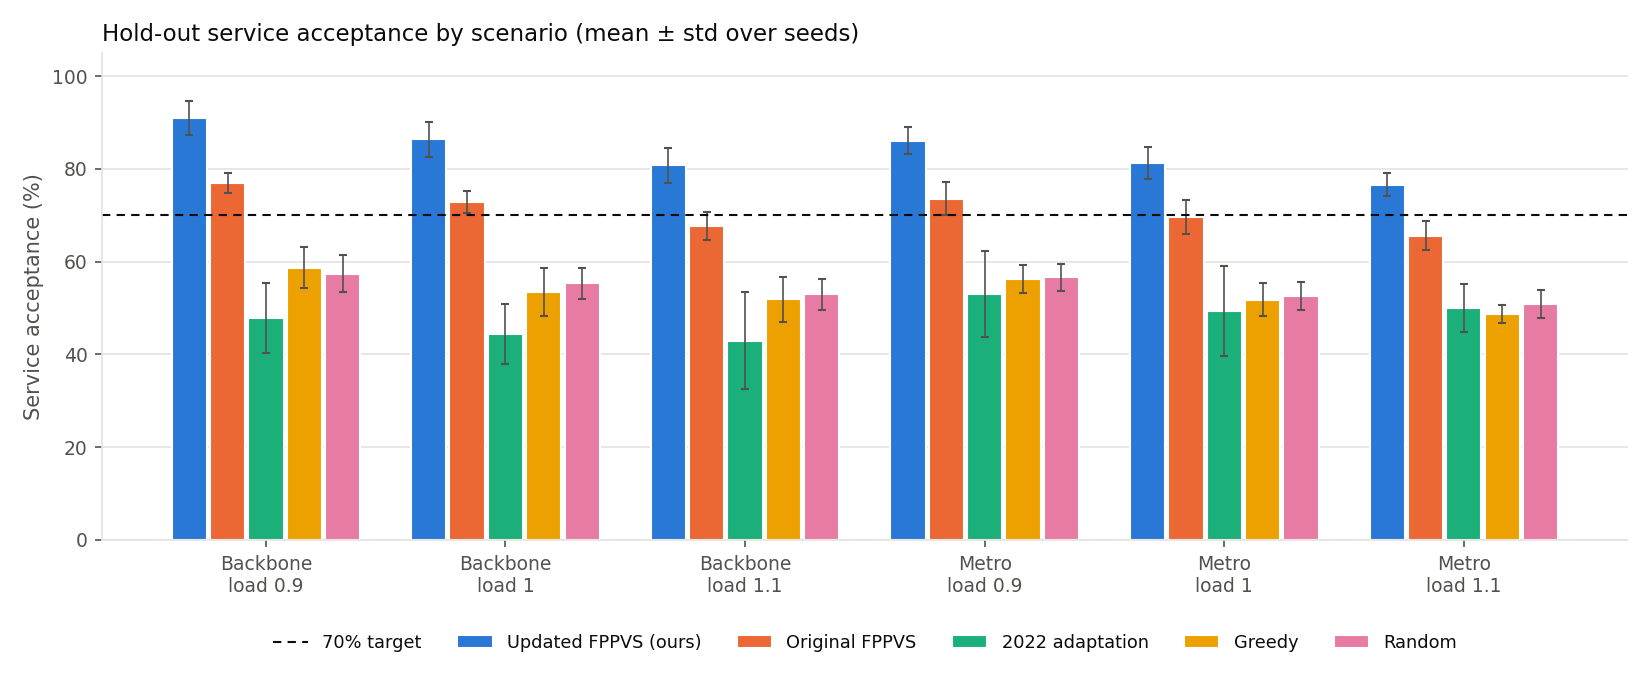
\includegraphics[width=\linewidth]{scenario-acceptance.png}
\caption{Hold-out acceptance in the six main scenarios. Error bars show one
standard deviation over seeds; the dashed line is the 70\% target.}
\label{fig:acc}
\end{figure}

\needspace{5\baselineskip}
\paragraph{Observations.}
\begin{itemize}
  \item Updated FPPVS is the best method in every scenario. At full load
  ($\rho=1$) it accepts 86.4\% on Backbone and 81.3\% on Metro, and even at 10\%
  overload ($\rho=1.1$) it still gets 80.8\% and 76.6\%.
  \item The original FPPVS is clearly second. It reaches
  \origMinAcc--\origMaxAcc\% in the main scenarios (mean \origMeanAcc\%) and
  beats the 2022 adaptation, greedy and random in every scenario, and in every
  one of the 30 main-scenario runs too; per scenario, its lead over the best of
  those three is 15--18 points. Its bandwidth pruning and neighbour rule keep
  chains compact, and its history signal pushes VNFs towards DCs that already
  run the same type. Updated FPPVS is \origGainMin--\origGainMax{} points above
  it (\origGainMean{} on average).
  \item The 2022 adaptation gets only \zhangMinAcc--\zhangMaxAcc\% (mean
  \zhangMeanAcc\%), which is below greedy and random in most scenarios. Greedy
  and random run with our feasibility mask, so they never pick a DC that is
  already known to break bandwidth or latency. The 2022 adaptation only checks
  compute while placing, as its method describes, and finds out about bandwidth
  and latency violations only when the whole chain is done (see Part E).
  \item The 2022 adaptation is also the least stable method: its standard
  deviation across seeds goes up to 10 points (Backbone, $\rho=1.1$). Getting
  just one reward value per episode (LTCR) gives the agent a weak learning
  signal.
  \item Greedy and random accept 49--59\%. They spread VNFs over a lot of DCs, so
  each request uses about twice as much link bandwidth as updated FPPVS
  (Section~C), and the links run out first.
  \item Metro is harder than Backbone at the same load. It has fewer DCs and
  fewer links, so when a link fills up there just aren't many other paths to
  use.
\end{itemize}

\begin{figure}[H]
\centering
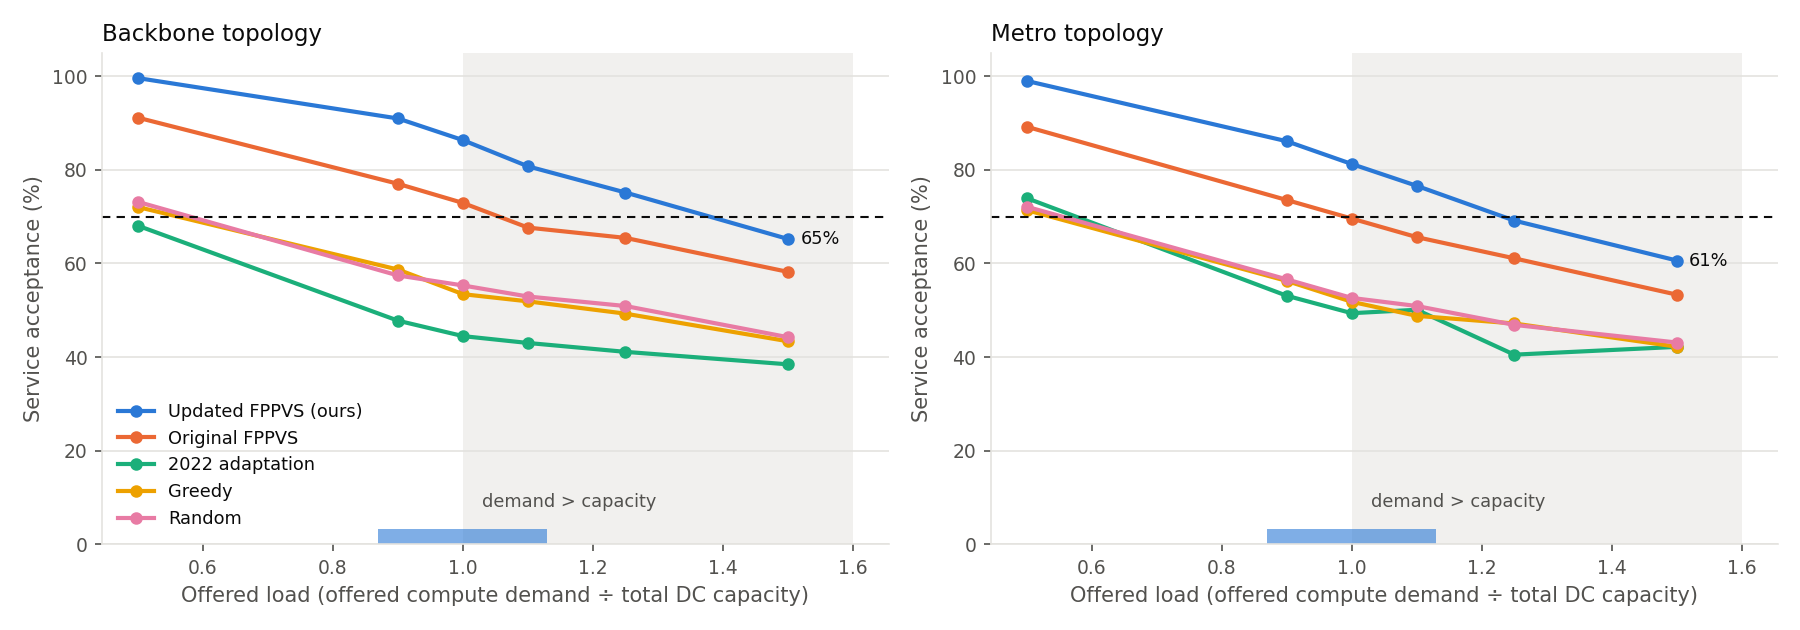
\includegraphics[width=\linewidth]{load-sweep.png}
\caption{Acceptance against offered load, from light load (0.5) to 50\%
overload (1.5). The shaded area is where the average offered compute is more
than the total compute of the network; the blue mark on the x-axis shows the
main scenarios.}
\label{fig:sweep}
\end{figure}

\paragraph{Load sweep.} Figure~\ref{fig:sweep} shows the full range of loads. At
light load ($\rho=0.5$), updated FPPVS accepts 99.6\% (Backbone) and 99.0\%
(Metro). This is kind of expected: with the network only half full, almost
every request fits as long as chains are kept compact, and the original FPPVS
also gets 91.2\% and 89.2\% there. That's why we use heavier loads as the main
scenarios. As the load goes up, acceptance drops smoothly: updated FPPVS gets
75.2\% and 69.2\% at $\rho=1.25$, and 65.2\% and 60.6\% at $\rho=1.5$. The
original FPPVS follows 7--10 points lower (53--66\%), and the 2022 adaptation,
greedy and random stay at or below 51\%. Going below 70\% can't be avoided in
this region: at $\rho=1.5$, only about two thirds of the offered compute can fit
in the network at any time, no matter what the placement policy is.

\subsubsection*{B. Ablation study}

\begin{table}[H]
\centering\small
\caption{Ablation: hold-out acceptance (\%) of updated FPPVS with one part
switched off at a time.}
\label{tab:ablation}
\begin{tabular}{lcccccc}
\toprule
Scenario & Full & w/o sharing & w/o fairness & 1 agent & w/o retry & Prior only \\
\midrule
Backbone 0.9 & 91.0 $\pm$ 3.6 & 78.7 $\pm$ 3.7 & 91.4 $\pm$ 3.2 & 90.9 $\pm$ 2.0 & 90.9 $\pm$ 2.8 & 91.9 $\pm$ 3.1 \\
Backbone 1 & 86.4 $\pm$ 3.7 & 73.8 $\pm$ 3.1 & 85.6 $\pm$ 3.9 & 86.0 $\pm$ 3.4 & 85.4 $\pm$ 3.1 & 86.3 $\pm$ 2.8 \\
Backbone 1.1 & 80.8 $\pm$ 3.8 & 68.2 $\pm$ 2.7 & 80.4 $\pm$ 4.1 & 81.2 $\pm$ 3.2 & 80.2 $\pm$ 3.5 & 80.9 $\pm$ 3.0 \\
Metro 0.9 & 86.1 $\pm$ 2.9 & 76.1 $\pm$ 2.1 & 86.8 $\pm$ 3.1 & 86.2 $\pm$ 3.0 & 86.0 $\pm$ 2.9 & 86.1 $\pm$ 3.1 \\
Metro 1 & 81.3 $\pm$ 3.5 & 70.6 $\pm$ 3.2 & 81.1 $\pm$ 2.9 & 81.0 $\pm$ 3.2 & 81.9 $\pm$ 4.0 & 81.7 $\pm$ 3.2 \\
Metro 1.1 & 76.6 $\pm$ 2.5 & 64.5 $\pm$ 2.8 & 75.7 $\pm$ 3.8 & 75.9 $\pm$ 3.8 & 76.4 $\pm$ 3.7 & 76.4 $\pm$ 2.9 \\
\bottomrule
\end{tabular}
\end{table}

Table~\ref{tab:ablation} turns off one part of updated FPPVS at a time.
\begin{itemize}
  \item \textbf{VNF sharing matters the most.} Without it, acceptance drops by
  10--13 points in every main scenario (for example 86.4\% to 73.8\% on Backbone
  at $\rho=1$). Every VNF then pays its own instance overhead, so the DCs fill up
  sooner.
  \item \textbf{Fairness bonus, single vs.\ federated training and retries}
  change acceptance by about one point or less, which is within the
  seed-to-seed spread. Fairness is meant to balance throughput between flows,
  not to push acceptance up, so this is expected. Retries only help in the rare
  case where the first placement runs into a dead end.
  \item \textbf{The learned network adds little over its prior.} ``Prior only''
  uses the same mask, prior and retries with no neural network at all, and it is
  within about one point of the full method everywhere. We're reporting this
  openly: in our experiments, the gains mostly come from the problem
  modifications (mask, sharing model, prior), not from the reinforcement
  learning itself. One reason is limitation L6: each episode covers only one
  request, so the agent doesn't see much of the long-term effect of its choices.
\end{itemize}

\subsubsection*{C. Resource usage}

Figure~\ref{fig:res} and Table~\ref{tab:res} show the resources each method holds
for the services it runs. Table~\ref{tab:savings} sums up the difference
between updated FPPVS and each of the other methods, averaged over the six main
scenarios.

\begin{figure}[H]
\centering
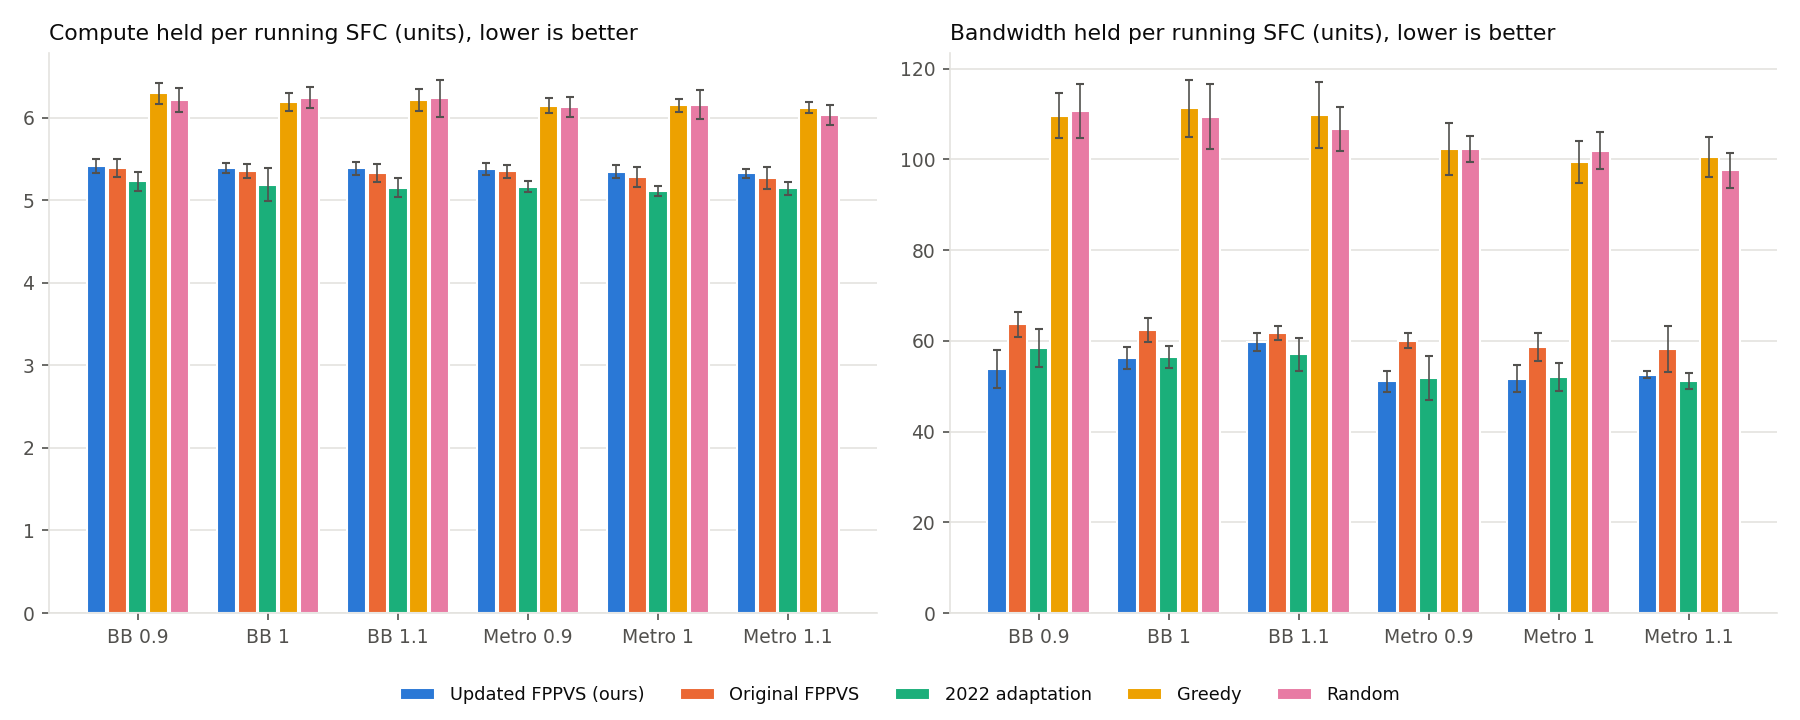
\includegraphics[width=\linewidth]{scenario-resources.png}
\caption{Compute (left) and bandwidth (right) held per running SFC, averaged over
time. Lower means each service costs less to keep running.}
\label{fig:res}
\end{figure}

\begin{table}[H]
\centering\small
\caption{Average reduction in resource use by updated FPPVS over each
method (main scenarios; positive means updated FPPVS uses less, negative means
it uses more).}
\label{tab:savings}
\begin{tabular}{lcccc}
\toprule
Reduction vs. & Compute & Bandwidth & BW$\cdot$time & Instances \\
 & per SFC & per SFC & per accepted & per accepted \\
\midrule
Original FPPVS & -0.8\% & +10.9\% & +11.0\% & +27.0\% \\
2022 adaptation & -4.0\% & +0.5\% & +2.1\% & +13.7\% \\
Greedy & +13.1\% & +48.7\% & +49.4\% & +91.8\% \\
Random & +12.9\% & +48.3\% & +48.6\% & +91.8\% \\
\bottomrule
\end{tabular}
\end{table}

\begin{table}[H]
\centering\scriptsize
\setlength{\tabcolsep}{4pt}
\caption{Resource use and latency per scenario (mean over seeds; best per
column within a scenario in bold). ``Per acc.'' means per accepted SFC.}
\label{tab:res}
\begin{tabular}{llcccccc}
\toprule
Scenario & Method & Compute & Bandwidth & Compute$\cdot$time & BW$\cdot$time & Instances & Latency \\
 & & per SFC & per SFC & per acc. ($10^3$) & per acc. ($10^3$) & per acc. & (ms) \\
\midrule
Backbone 0.9 & Updated (ours) & 5.42 & \textbf{53.8} & 5.43 & \textbf{54.0} & \textbf{0.57} & \textbf{46.5} \\
 & Original FPPVS & 5.39 & 63.7 & \textbf{5.32} & 62.9 & 0.78 & 56.0 \\
 & 2022 adaptation & \textbf{5.23} & 58.4 & 5.37 & 60.0 & 0.59 & 66.2 \\
 & Greedy & 6.29 & 109.6 & 6.31 & 109.8 & 6.66 & 107.8 \\
 & Random & 6.22 & 110.7 & 6.40 & 114.0 & 6.57 & 108.8 \\
\midrule
Backbone 1 & Updated (ours) & 5.39 & \textbf{56.2} & 5.42 & \textbf{56.5} & \textbf{0.53} & \textbf{50.0} \\
 & Original FPPVS & 5.35 & 62.3 & 5.40 & 62.9 & 0.73 & 56.2 \\
 & 2022 adaptation & \textbf{5.19} & 56.5 & \textbf{5.28} & 57.4 & 0.61 & 67.2 \\
 & Greedy & 6.19 & 111.2 & 6.40 & 115.1 & 6.58 & 107.7 \\
 & Random & 6.24 & 109.4 & 6.27 & 110.1 & 6.58 & 108.1 \\
\midrule
Backbone 1.1 & Updated (ours) & 5.39 & 59.6 & 5.40 & 59.9 & \textbf{0.52} & \textbf{53.2} \\
 & Original FPPVS & 5.33 & 61.7 & 5.37 & 62.2 & 0.74 & 54.7 \\
 & 2022 adaptation & \textbf{5.15} & \textbf{57.0} & \textbf{5.26} & \textbf{58.2} & 0.63 & 70.2 \\
 & Greedy & 6.21 & 109.9 & 6.30 & 111.5 & 6.59 & 107.4 \\
 & Random & 6.23 & 106.7 & 6.24 & 107.0 & 6.56 & 108.8 \\
\midrule
Metro 0.9 & Updated (ours) & 5.38 & \textbf{51.1} & 5.50 & \textbf{52.3} & \textbf{0.55} & \textbf{45.8} \\
 & Original FPPVS & 5.35 & 60.0 & 5.44 & 61.1 & 0.74 & 54.5 \\
 & 2022 adaptation & \textbf{5.17} & 51.8 & \textbf{5.28} & 53.1 & 0.67 & 65.5 \\
 & Greedy & 6.15 & 102.2 & 6.27 & 104.6 & 6.56 & 105.2 \\
 & Random & 6.13 & 102.2 & 6.22 & 103.9 & 6.47 & 105.9 \\
\midrule
Metro 1 & Updated (ours) & 5.35 & \textbf{51.6} & 5.44 & \textbf{52.5} & \textbf{0.55} & \textbf{48.6} \\
 & Original FPPVS & 5.28 & 58.7 & 5.46 & 60.7 & 0.71 & 54.1 \\
 & 2022 adaptation & \textbf{5.11} & 52.0 & \textbf{5.35} & 54.4 & 0.62 & 67.2 \\
 & Greedy & 6.15 & 99.4 & 6.46 & 104.4 & 6.53 & 104.1 \\
 & Random & 6.16 & 101.9 & 6.38 & 105.6 & 6.51 & 105.2 \\
\midrule
Metro 1.1 & Updated (ours) & 5.33 & 52.6 & 5.43 & 53.6 & \textbf{0.51} & \textbf{50.2} \\
 & Original FPPVS & 5.28 & 58.3 & 5.37 & 59.3 & 0.71 & 54.2 \\
 & 2022 adaptation & \textbf{5.14} & \textbf{51.2} & \textbf{5.32} & \textbf{53.0} & 0.63 & 65.2 \\
 & Greedy & 6.12 & 100.5 & 6.34 & 104.1 & 6.52 & 105.0 \\
 & Random & 6.03 & 97.6 & 6.14 & 99.4 & 6.41 & 104.0 \\
\bottomrule
\end{tabular}
\end{table}

\needspace{5\baselineskip}
\paragraph{Observations.}
\begin{itemize}
  \item \textbf{Coming to bandwidth:} updated FPPVS holds about half the link
  bandwidth per running SFC compared to greedy and random (48--49\% less), and
  11\% less than the original FPPVS. Against the 2022 adaptation it's about
  even: 0.5\% less on average, lower at $\rho=0.9$ and $\rho=1.0$, and a bit
  higher at $\rho=1.1$. But keep in mind that updated FPPVS carries 1.5--1.9
  times as many requests as the 2022 adaptation at the same time, including
  harder ones that the other method rejects.
  \item \textbf{Coming to instances:} updated FPPVS starts 0.51--0.57 new VNF
  instances per accepted request. That is 27\% fewer than the original FPPVS
  (0.71--0.78), 14\% fewer than the 2022 adaptation, and about 92\% fewer than
  greedy and random (about 6.6, one per VNF, since they don't share). The
  placement prior's reuse term is the main reason for this.
  \item \textbf{Coming to compute:} against greedy and random, it needs about
  13\% less compute per service, because it shares instances. Against the
  original FPPVS it's about the same (within 1\%). Against the 2022 adaptation
  it uses about 4\% more. But that method accepts far fewer requests, most
  likely the easier ones, so its per-request average comes from an easier set.
  \item \textbf{Coming to latency:} mean latency of accepted requests is
  46--53\,ms for updated FPPVS, 54--56\,ms for the original FPPVS, 65--70\,ms for
  the 2022 adaptation, and 104--108\,ms for greedy and random. All of them are
  under the 100--150\,ms limits. The 2022 adaptation places the chain strictly in
  sequence (no parallel branches), so every monitor adds to the critical path.
  \item \textbf{Decision time and training.} Updated FPPVS needs 9--13\,ms per
  request, including the CNN forward pass and the occasional retry; the original
  FPPVS needs 17--28\,ms, because its fully connected layer takes in the whole
  feature map; the 2022 adaptation needs 4--5\,ms; and greedy and random need
  2--3\,ms. Training one updated FPPVS model with 2000 episodes takes about
  \trainSeconds\,s on the CPU, and one original FPPVS model takes about
  200--400\,s.
\end{itemize}

\subsubsection*{D. Effect of the algorithm alone}

Our main experiments use a different arrival process from our first version
(modification M1). So to separate the effect of the algorithm from the effect of
the workload, we also ran the updated placement logic on the original workload:
one arrival per time unit, 100 requests, with almost nothing released during the
run (Table~\ref{tab:old}). The updated placement gets 70.4\%, up from 10.4\% for
the original implementation. Acceptance is lower than in the Poisson runs mainly
because the original stream throws far more traffic at the network than it can
hold.

\begin{table}[H]
\centering\small
\caption{Original workload (one arrival per time unit), 5 seeds. The upper
rows are from our first implementation; the lower rows use the updated
environment and placement logic.}
\label{tab:old}
\begin{tabular}{lc}
\toprule
Method (original workload, 100 requests) & Acceptance (\%) \\
\midrule
Original implementation, trained FDRL (5 seeds) & 10.4 $\pm$ 5.1 \\
Original implementation, greedy & 15.8 $\pm$ 3.1 \\
Original implementation, random & 11.6 $\pm$ 3.0 \\
\midrule
Updated FPPVS placement & 70.4 $\pm$ 2.9 \\
Greedy & 45.4 $\pm$ 2.1 \\
Random & 46.2 $\pm$ 2.2 \\
\bottomrule
\end{tabular}
\end{table}

\subsubsection*{E. Comparison with the original FPPVS and the 2022 adaptation}\label{sec:paper}

\paragraph{Same scenarios, same requests.} Table~\ref{tab:orig} puts the three
learning-based methods side by side. All three get 2000 training episodes and
are tested on the same hold-out requests.

\begin{table}[H]
\centering\small
\caption{Original FPPVS, the 2022 adaptation and updated FPPVS on identical
scenarios, mean over \numSeeds{} seeds. $^\ast$Gain = updated FPPVS minus the
better of the other two, in percentage points.}
\label{tab:orig}
\begin{tabular}{lccccccc}
\toprule
 & \multicolumn{4}{c}{Acceptance (\%)} & \multicolumn{3}{c}{Bandwidth per running SFC} \\
\cmidrule(lr){2-5}\cmidrule(lr){6-8}
Scenario & Original & 2022 & Updated & Gain$^\ast$ & Original & 2022 & Updated \\
\midrule
Backbone 0.9 & 77.0 & 47.8 & \textbf{91.0} & +14.0 & 63.7 & 58.4 & \textbf{53.8} \\
Backbone 1 & 72.9 & 44.5 & \textbf{86.4} & +13.4 & 62.3 & 56.5 & \textbf{56.2} \\
Backbone 1.1 & 67.7 & 43.0 & \textbf{80.8} & +13.1 & 61.7 & 57.0 & \textbf{59.6} \\
Metro 0.9 & 73.6 & 53.1 & \textbf{86.1} & +12.6 & 60.0 & 51.8 & \textbf{51.1} \\
Metro 1 & 69.6 & 49.4 & \textbf{81.3} & +11.7 & 58.7 & 52.0 & \textbf{51.6} \\
Metro 1.1 & 65.6 & 50.1 & \textbf{76.6} & +11.0 & 58.3 & 51.2 & \textbf{52.6} \\
\midrule \multicolumn{8}{l}{\emph{Other load levels}} \\
Backbone 0.5 & 91.2 & 68.1 & \textbf{99.6} & +8.5 & 65.5 & 57.6 & \textbf{40.5} \\
Backbone 1.25 & 65.5 & 41.1 & \textbf{75.2} & +9.7 & 61.1 & 57.1 & \textbf{59.9} \\
Backbone 1.5 & 58.2 & 38.4 & \textbf{65.2} & +7.0 & 60.1 & 57.8 & \textbf{59.5} \\
Metro 0.5 & 89.2 & 74.0 & \textbf{99.0} & +9.8 & 60.5 & 52.9 & \textbf{41.0} \\
Metro 1.25 & 61.1 & 40.5 & \textbf{69.2} & +8.1 & 58.8 & 52.2 & \textbf{55.4} \\
Metro 1.5 & 53.3 & 42.2 & \textbf{60.6} & +7.3 & 58.6 & 51.7 & \textbf{55.9} \\
\bottomrule
\end{tabular}
\end{table}

\begin{itemize}
  \item Updated FPPVS accepts 11--14 percentage points more than the original
  FPPVS in the main scenarios, and 7--10 points more at the other load levels.
  The original, in turn, is 16--29 points above the 2022 adaptation.
  \item The other two learning methods fail in different ways. Almost all of the
  original FPPVS's rejections (96--98\%) are dead ends: after the previous VNF is
  placed, no neighbouring node has enough compute and bandwidth for the next one.
  Only 2--4\% are latency violations found at the end. The 2022 adaptation only
  checks compute, so 63--70\% of its rejections are link bandwidth and 30--37\%
  are latency, and all of them are found only after the whole chain is placed.
  It has more latency failures because it doesn't parallelize monitors.
  \item Updated FPPVS gets rid of both problems. Its look-ahead mask checks
  compute, bandwidth and the latency bound on every DC, not just on neighbours,
  and its placement prior looks ahead to the destination, so it rarely walks
  into a dead end. And if it does, rollback-and-retry tries another first DC
  (limitation L3).
  \item How closely you follow the paper matters a lot. An earlier, looser
  reading of the original (pruning by compute only, any DC as a candidate, and
  global pooling in the CNN) got only 41--50\% on the same scenarios. Following
  Section 4.3 closely pushed it up to \origMinAcc--\origMaxAcc\%.
\end{itemize}

\paragraph{Published numbers.} Table~\ref{tab:paper} shows the results published
in the FPPVS paper next to our three runs at full load ($\rho=1$).

\begin{table}[H]
\centering\small
\caption{Published FPPVS results (Tables 6 and 7 of the paper) next to our runs
of the original FPPVS, the 2022 adaptation and updated FPPVS at load 1.0. Values
come from different data and settings; see the text before comparing them.}
\label{tab:paper}
\begin{tabular}{llcccc}
\toprule
 & & Published & \multicolumn{3}{c}{Our runs, load 1.0} \\
\cmidrule(lr){4-6}
Topology & Metric & FPPVS (paper) & Original & 2022 & Updated \\
\midrule
Backbone & Acceptance (\%) & 88.1 & 72.9 & 44.5 & 86.4 \\
 & Latency (ms) & 134.4 & 56.2 & 67.2 & 50.0 \\
 & Resource utilization (\%) & 75.35 & 70.4 & 42.3 & 82.8 \\
\midrule
Metro & Acceptance (\%) & 75.9 & 69.6 & 49.4 & 81.3 \\
 & Latency (ms) & 160.1 & 54.1 & 67.2 & 48.6 \\
 & Resource utilization (\%) & 72.36 & 70.6 & 49.4 & 82.5 \\
\bottomrule
\end{tabular}
\end{table}

Our run of the original specification gets 72.9\% (Backbone) and 69.6\%
(Metro), against the 88.1\% and 75.9\% the paper reports. The Metro value is
close, but the Backbone value is about 15 points lower. We would say there are
four likely reasons for the gap that's left:
\begin{enumerate}
  \item \textbf{Workload.} The paper's arrival rate is not given (L1). Its
  numbers may come from a lighter load than our $\rho=1$.
  \item \textbf{Data.} The paper uses the real USAnet and Italian operator
  topologies and traces (L2), while we use random graphs of the same size.
  \item \textbf{Training budget.} The paper trains for 2000 iterations of 10
  episodes with 20 SFCs each, so about 400{,}000 SFC placements. Our models see
  2000 episodes (one SFC each) on a laptop CPU.
  \item \textbf{Unstated details.} A few parts of the original method aren't
  fully described (sharing capacity, exact state encoding, final-reward scale),
  so our reading of them may be different from the authors' code.
\end{enumerate}
Latency and utilization are also defined differently. Our latency counts link
delay and VNF processing on the critical path, and the paper's values (above
100\,ms) kind of suggest it includes more delay components. Our utilization is
the time-averaged share of total compute in use. So these rows only show
trends.

What the comparison does show is consistent: under the same heavy-load
conditions, mean acceptance in the main scenarios is \zhangMeanAcc\% for the 2022
adaptation, \origMeanAcc\% for the original FPPVS and \fppvsMeanAcc\% for updated
FPPVS. At full load, updated FPPVS (86.4\% and 81.3\%) is in the same range as
the paper's published values (88.1\% and 75.9\%).
